% Options for packages loaded elsewhere
\PassOptionsToPackage{unicode}{hyperref}
\PassOptionsToPackage{hyphens}{url}
%
\documentclass[
]{article}
\usepackage{amsmath,amssymb}
\usepackage{lmodern}
\usepackage{ifxetex,ifluatex}
\ifnum 0\ifxetex 1\fi\ifluatex 1\fi=0 % if pdftex
  \usepackage[T1]{fontenc}
  \usepackage[utf8]{inputenc}
  \usepackage{textcomp} % provide euro and other symbols
\else % if luatex or xetex
  \usepackage{unicode-math}
  \defaultfontfeatures{Scale=MatchLowercase}
  \defaultfontfeatures[\rmfamily]{Ligatures=TeX,Scale=1}
\fi
% Use upquote if available, for straight quotes in verbatim environments
\IfFileExists{upquote.sty}{\usepackage{upquote}}{}
\IfFileExists{microtype.sty}{% use microtype if available
  \usepackage[]{microtype}
  \UseMicrotypeSet[protrusion]{basicmath} % disable protrusion for tt fonts
}{}
\makeatletter
\@ifundefined{KOMAClassName}{% if non-KOMA class
  \IfFileExists{parskip.sty}{%
    \usepackage{parskip}
  }{% else
    \setlength{\parindent}{0pt}
    \setlength{\parskip}{6pt plus 2pt minus 1pt}}
}{% if KOMA class
  \KOMAoptions{parskip=half}}
\makeatother
\usepackage{xcolor}
\IfFileExists{xurl.sty}{\usepackage{xurl}}{} % add URL line breaks if available
\IfFileExists{bookmark.sty}{\usepackage{bookmark}}{\usepackage{hyperref}}
\hypersetup{
  pdftitle={class12: Structural Bioinformatics II},
  pdfauthor={Anel A15426506},
  hidelinks,
  pdfcreator={LaTeX via pandoc}}
\urlstyle{same} % disable monospaced font for URLs
\usepackage[margin=1in]{geometry}
\usepackage{color}
\usepackage{fancyvrb}
\newcommand{\VerbBar}{|}
\newcommand{\VERB}{\Verb[commandchars=\\\{\}]}
\DefineVerbatimEnvironment{Highlighting}{Verbatim}{commandchars=\\\{\}}
% Add ',fontsize=\small' for more characters per line
\usepackage{framed}
\definecolor{shadecolor}{RGB}{248,248,248}
\newenvironment{Shaded}{\begin{snugshade}}{\end{snugshade}}
\newcommand{\AlertTok}[1]{\textcolor[rgb]{0.94,0.16,0.16}{#1}}
\newcommand{\AnnotationTok}[1]{\textcolor[rgb]{0.56,0.35,0.01}{\textbf{\textit{#1}}}}
\newcommand{\AttributeTok}[1]{\textcolor[rgb]{0.77,0.63,0.00}{#1}}
\newcommand{\BaseNTok}[1]{\textcolor[rgb]{0.00,0.00,0.81}{#1}}
\newcommand{\BuiltInTok}[1]{#1}
\newcommand{\CharTok}[1]{\textcolor[rgb]{0.31,0.60,0.02}{#1}}
\newcommand{\CommentTok}[1]{\textcolor[rgb]{0.56,0.35,0.01}{\textit{#1}}}
\newcommand{\CommentVarTok}[1]{\textcolor[rgb]{0.56,0.35,0.01}{\textbf{\textit{#1}}}}
\newcommand{\ConstantTok}[1]{\textcolor[rgb]{0.00,0.00,0.00}{#1}}
\newcommand{\ControlFlowTok}[1]{\textcolor[rgb]{0.13,0.29,0.53}{\textbf{#1}}}
\newcommand{\DataTypeTok}[1]{\textcolor[rgb]{0.13,0.29,0.53}{#1}}
\newcommand{\DecValTok}[1]{\textcolor[rgb]{0.00,0.00,0.81}{#1}}
\newcommand{\DocumentationTok}[1]{\textcolor[rgb]{0.56,0.35,0.01}{\textbf{\textit{#1}}}}
\newcommand{\ErrorTok}[1]{\textcolor[rgb]{0.64,0.00,0.00}{\textbf{#1}}}
\newcommand{\ExtensionTok}[1]{#1}
\newcommand{\FloatTok}[1]{\textcolor[rgb]{0.00,0.00,0.81}{#1}}
\newcommand{\FunctionTok}[1]{\textcolor[rgb]{0.00,0.00,0.00}{#1}}
\newcommand{\ImportTok}[1]{#1}
\newcommand{\InformationTok}[1]{\textcolor[rgb]{0.56,0.35,0.01}{\textbf{\textit{#1}}}}
\newcommand{\KeywordTok}[1]{\textcolor[rgb]{0.13,0.29,0.53}{\textbf{#1}}}
\newcommand{\NormalTok}[1]{#1}
\newcommand{\OperatorTok}[1]{\textcolor[rgb]{0.81,0.36,0.00}{\textbf{#1}}}
\newcommand{\OtherTok}[1]{\textcolor[rgb]{0.56,0.35,0.01}{#1}}
\newcommand{\PreprocessorTok}[1]{\textcolor[rgb]{0.56,0.35,0.01}{\textit{#1}}}
\newcommand{\RegionMarkerTok}[1]{#1}
\newcommand{\SpecialCharTok}[1]{\textcolor[rgb]{0.00,0.00,0.00}{#1}}
\newcommand{\SpecialStringTok}[1]{\textcolor[rgb]{0.31,0.60,0.02}{#1}}
\newcommand{\StringTok}[1]{\textcolor[rgb]{0.31,0.60,0.02}{#1}}
\newcommand{\VariableTok}[1]{\textcolor[rgb]{0.00,0.00,0.00}{#1}}
\newcommand{\VerbatimStringTok}[1]{\textcolor[rgb]{0.31,0.60,0.02}{#1}}
\newcommand{\WarningTok}[1]{\textcolor[rgb]{0.56,0.35,0.01}{\textbf{\textit{#1}}}}
\usepackage{graphicx}
\makeatletter
\def\maxwidth{\ifdim\Gin@nat@width>\linewidth\linewidth\else\Gin@nat@width\fi}
\def\maxheight{\ifdim\Gin@nat@height>\textheight\textheight\else\Gin@nat@height\fi}
\makeatother
% Scale images if necessary, so that they will not overflow the page
% margins by default, and it is still possible to overwrite the defaults
% using explicit options in \includegraphics[width, height, ...]{}
\setkeys{Gin}{width=\maxwidth,height=\maxheight,keepaspectratio}
% Set default figure placement to htbp
\makeatletter
\def\fps@figure{htbp}
\makeatother
\setlength{\emergencystretch}{3em} % prevent overfull lines
\providecommand{\tightlist}{%
  \setlength{\itemsep}{0pt}\setlength{\parskip}{0pt}}
\setcounter{secnumdepth}{-\maxdimen} % remove section numbering
\ifluatex
  \usepackage{selnolig}  % disable illegal ligatures
\fi

\title{class12: Structural Bioinformatics II}
\author{Anel A15426506}
\date{11/4/2021}

\begin{document}
\maketitle

\#Comparative analysis of protein structures

using the bio3d package

\begin{Shaded}
\begin{Highlighting}[]
\FunctionTok{library}\NormalTok{(bio3d)}

\NormalTok{pdb }\OtherTok{\textless{}{-}} \FunctionTok{read.pdb}\NormalTok{(}\StringTok{"1hel"}\NormalTok{)}
\end{Highlighting}
\end{Shaded}

\begin{verbatim}
##   Note: Accessing on-line PDB file
\end{verbatim}

\begin{Shaded}
\begin{Highlighting}[]
\NormalTok{pdb}
\end{Highlighting}
\end{Shaded}

\begin{verbatim}
## 
##  Call:  read.pdb(file = "1hel")
## 
##    Total Models#: 1
##      Total Atoms#: 1186,  XYZs#: 3558  Chains#: 1  (values: A)
## 
##      Protein Atoms#: 1001  (residues/Calpha atoms#: 129)
##      Nucleic acid Atoms#: 0  (residues/phosphate atoms#: 0)
## 
##      Non-protein/nucleic Atoms#: 185  (residues: 185)
##      Non-protein/nucleic resid values: [ HOH (185) ]
## 
##    Protein sequence:
##       KVFGRCELAAAMKRHGLDNYRGYSLGNWVCAAKFESNFNTQATNRNTDGSTDYGILQINS
##       RWWCNDGRTPGSRNLCNIPCSALLSSDITASVNCAKKIVSDGNGMNAWVAWRNRCKGTDV
##       QAWIRGCRL
## 
## + attr: atom, xyz, seqres, helix, sheet,
##         calpha, remark, call
\end{verbatim}

let's use a bioinformarics method called NMA (Normal Mode ANalysis) to
predict the dynamics (flexibilty) of this enzyme.

\begin{Shaded}
\begin{Highlighting}[]
\NormalTok{modes }\OtherTok{\textless{}{-}} \FunctionTok{nma}\NormalTok{(pdb)}
\end{Highlighting}
\end{Shaded}

\begin{verbatim}
##  Building Hessian...     Done in 0.021 seconds.
##  Diagonalizing Hessian...    Done in 0.118 seconds.
\end{verbatim}

\begin{Shaded}
\begin{Highlighting}[]
\FunctionTok{plot}\NormalTok{(modes)}
\end{Highlighting}
\end{Shaded}

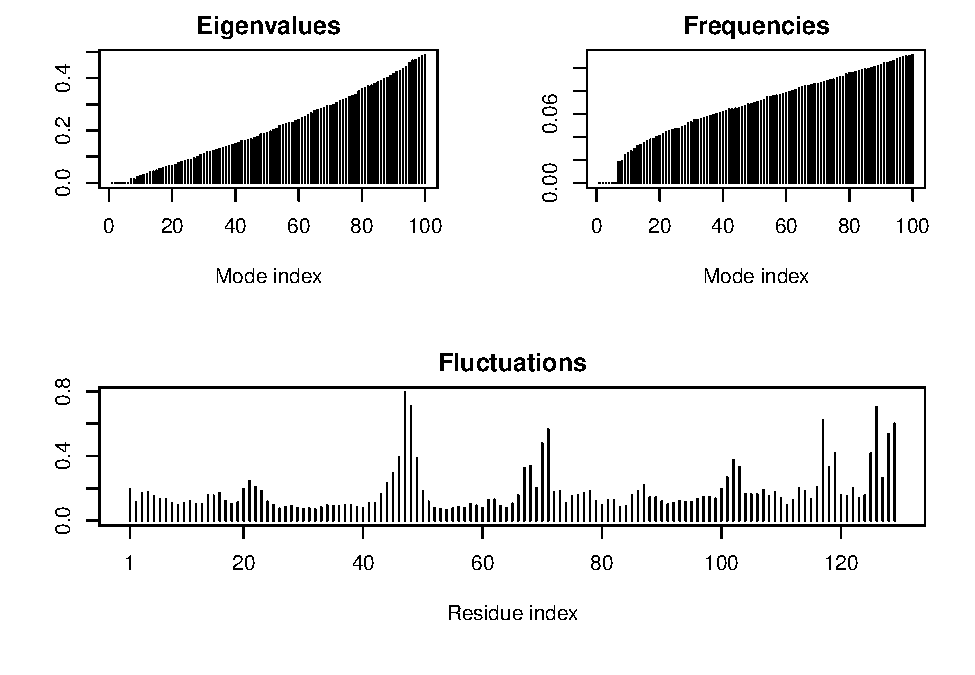
\includegraphics{class-12_files/figure-latex/unnamed-chunk-2-1.pdf}

make a ``move'' of its predicted motion. we often call this a
``trajectory''

\begin{Shaded}
\begin{Highlighting}[]
\FunctionTok{mktrj}\NormalTok{(modes, }\AttributeTok{file=}\StringTok{"nma.pdb"}\NormalTok{)}
\end{Highlighting}
\end{Shaded}

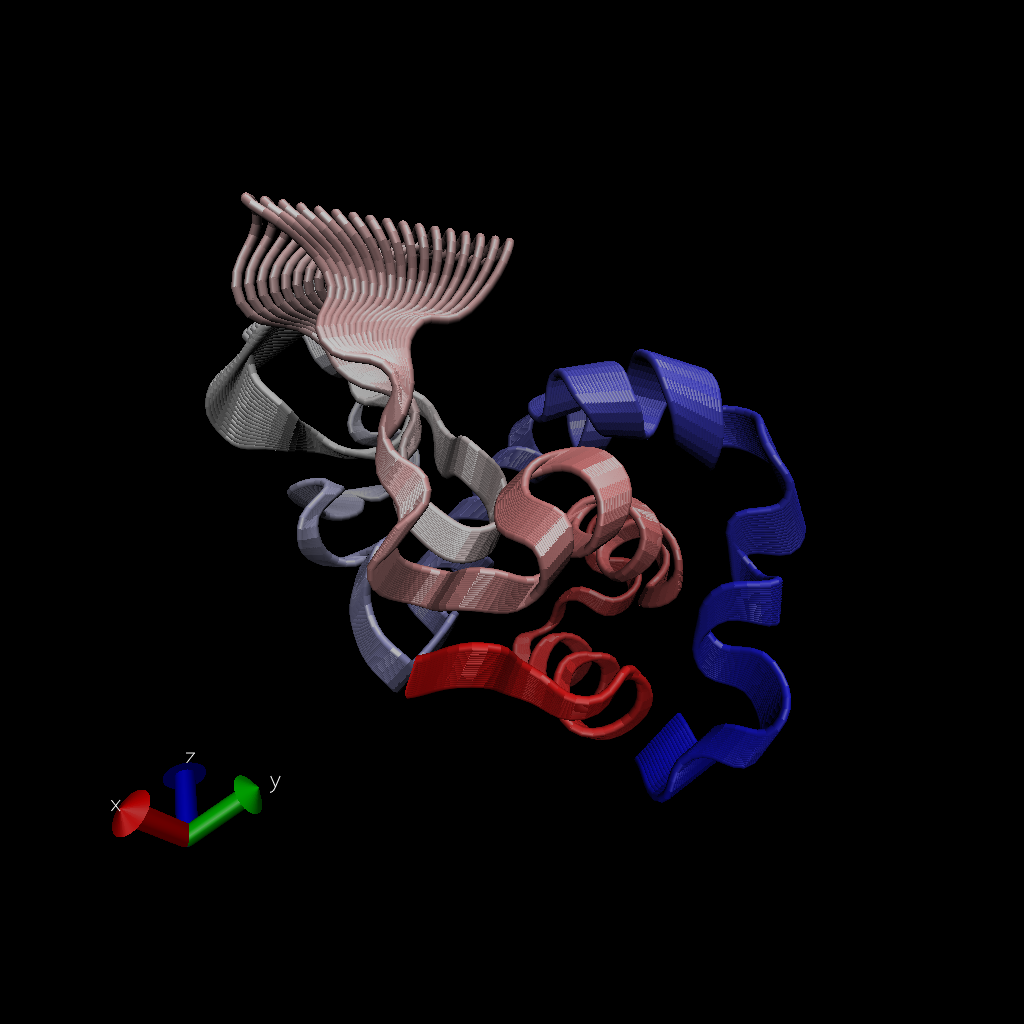
\includegraphics{vmdscene.bmp}

\begin{Shaded}
\begin{Highlighting}[]
\NormalTok{hits }\OtherTok{\textless{}{-}} \ConstantTok{NULL}
\NormalTok{hits}\SpecialCharTok{$}\NormalTok{pdb.id }\OtherTok{\textless{}{-}} \FunctionTok{c}\NormalTok{(}\StringTok{\textquotesingle{}1AKE\_A\textquotesingle{}}\NormalTok{,}\StringTok{\textquotesingle{}4X8M\_A\textquotesingle{}}\NormalTok{,}\StringTok{\textquotesingle{}6S36\_A\textquotesingle{}}\NormalTok{,}\StringTok{\textquotesingle{}6RZE\_A\textquotesingle{}}\NormalTok{,}\StringTok{\textquotesingle{}4X8H\_A\textquotesingle{}}\NormalTok{,}\StringTok{\textquotesingle{}3HPR\_A\textquotesingle{}}\NormalTok{,}\StringTok{\textquotesingle{}1E4V\_A\textquotesingle{}}\NormalTok{,}\StringTok{\textquotesingle{}5EJE\_A\textquotesingle{}}\NormalTok{,}\StringTok{\textquotesingle{}1E4Y\_A\textquotesingle{}}\NormalTok{,}\StringTok{\textquotesingle{}3X2S\_A\textquotesingle{}}\NormalTok{,}\StringTok{\textquotesingle{}6HAP\_A\textquotesingle{}}\NormalTok{,}\StringTok{\textquotesingle{}6HAM\_A\textquotesingle{}}\NormalTok{,}\StringTok{\textquotesingle{}4K46\_A\textquotesingle{}}\NormalTok{,}\StringTok{\textquotesingle{}4NP6\_A\textquotesingle{}}\NormalTok{,}\StringTok{\textquotesingle{}3GMT\_A\textquotesingle{}}\NormalTok{,}\StringTok{\textquotesingle{}4PZL\_A\textquotesingle{}}\NormalTok{)}
\end{Highlighting}
\end{Shaded}

\hypertarget{download-pdb-files}{%
\section{download PDB files}\label{download-pdb-files}}

\begin{Shaded}
\begin{Highlighting}[]
\CommentTok{\#files \textless{}{-} get.pdb(hits$pdb.id, path="pdbs", split=TRUE, gzip=TRUE)}
\end{Highlighting}
\end{Shaded}

Multiple structure alignment

\begin{Shaded}
\begin{Highlighting}[]
\CommentTok{\#pdb \textless{}{-} pdbaln(files, fit= TRUE)}
\end{Highlighting}
\end{Shaded}

\begin{Shaded}
\begin{Highlighting}[]
\NormalTok{pdb}
\end{Highlighting}
\end{Shaded}

\begin{verbatim}
## 
##  Call:  read.pdb(file = "1hel")
## 
##    Total Models#: 1
##      Total Atoms#: 1186,  XYZs#: 3558  Chains#: 1  (values: A)
## 
##      Protein Atoms#: 1001  (residues/Calpha atoms#: 129)
##      Nucleic acid Atoms#: 0  (residues/phosphate atoms#: 0)
## 
##      Non-protein/nucleic Atoms#: 185  (residues: 185)
##      Non-protein/nucleic resid values: [ HOH (185) ]
## 
##    Protein sequence:
##       KVFGRCELAAAMKRHGLDNYRGYSLGNWVCAAKFESNFNTQATNRNTDGSTDYGILQINS
##       RWWCNDGRTPGSRNLCNIPCSALLSSDITASVNCAKKIVSDGNGMNAWVAWRNRCKGTDV
##       QAWIRGCRL
## 
## + attr: atom, xyz, seqres, helix, sheet,
##         calpha, remark, call
\end{verbatim}

\begin{Shaded}
\begin{Highlighting}[]
\CommentTok{\#ids \textless{}{-} basename.pdb(pdb$id)}
\end{Highlighting}
\end{Shaded}

\begin{Shaded}
\begin{Highlighting}[]
\CommentTok{\#plot(pdb, labels=ids)}
\end{Highlighting}
\end{Shaded}

we will use the bio3d pca() function which is designed for protein
structure data.

\begin{Shaded}
\begin{Highlighting}[]
\CommentTok{\#pc.xray \textless{}{-} pca(pdb)}
\CommentTok{\#plot(pc.xray)}
\end{Highlighting}
\end{Shaded}

make a trajectory vsiualization of the motion captured by the first
Principal component

\hypertarget{visualize-first-principal-component}{%
\section{Visualize first principal
component}\label{visualize-first-principal-component}}

\begin{Shaded}
\begin{Highlighting}[]
\CommentTok{\#pc1 \textless{}{-} mktrj(pc.xray, pc=1, file="pc\_1.pdb")}
\end{Highlighting}
\end{Shaded}

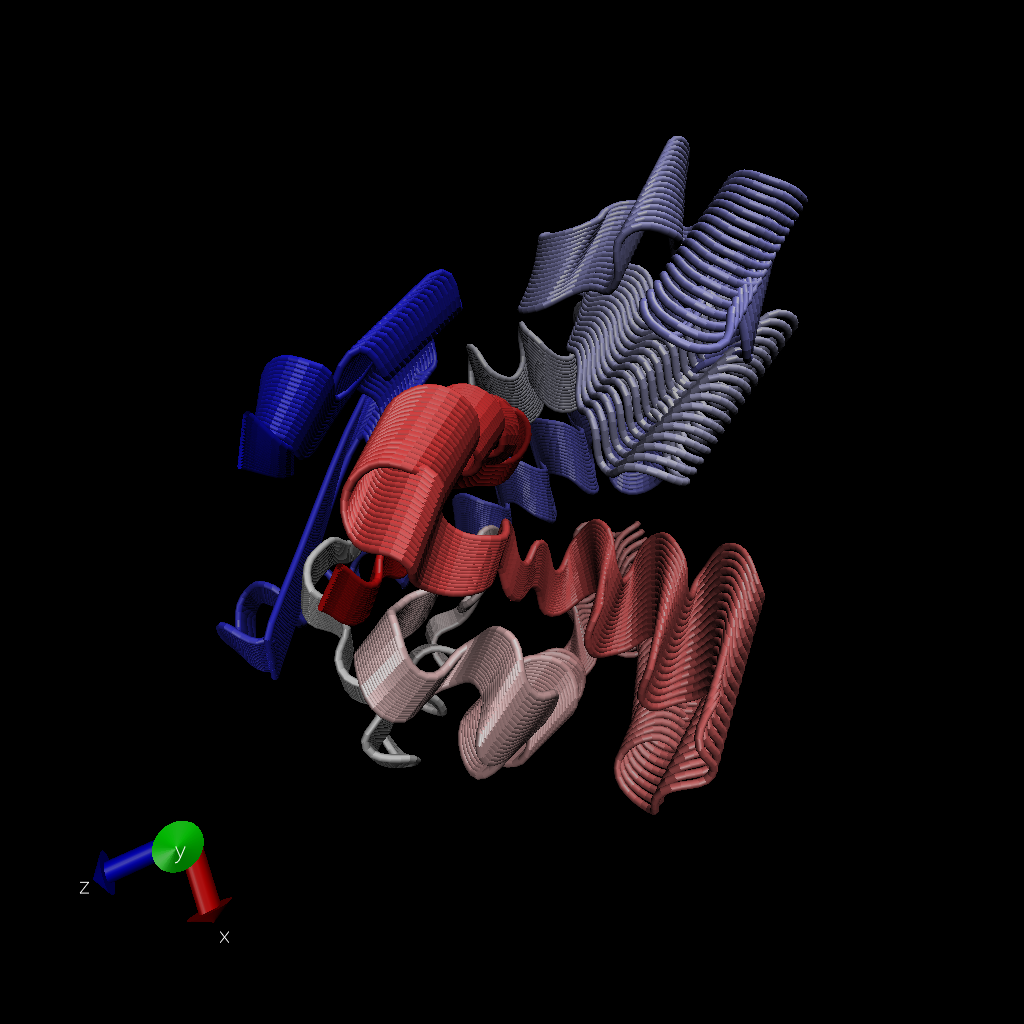
\includegraphics{pc_1.bmp}

\end{document}
